\subsection{QuizziPedia::Back-End}
\subsubsection{Informazioni generali}
\label{QuizziPedia::Back-End}
\begin{figure}
	\centering
	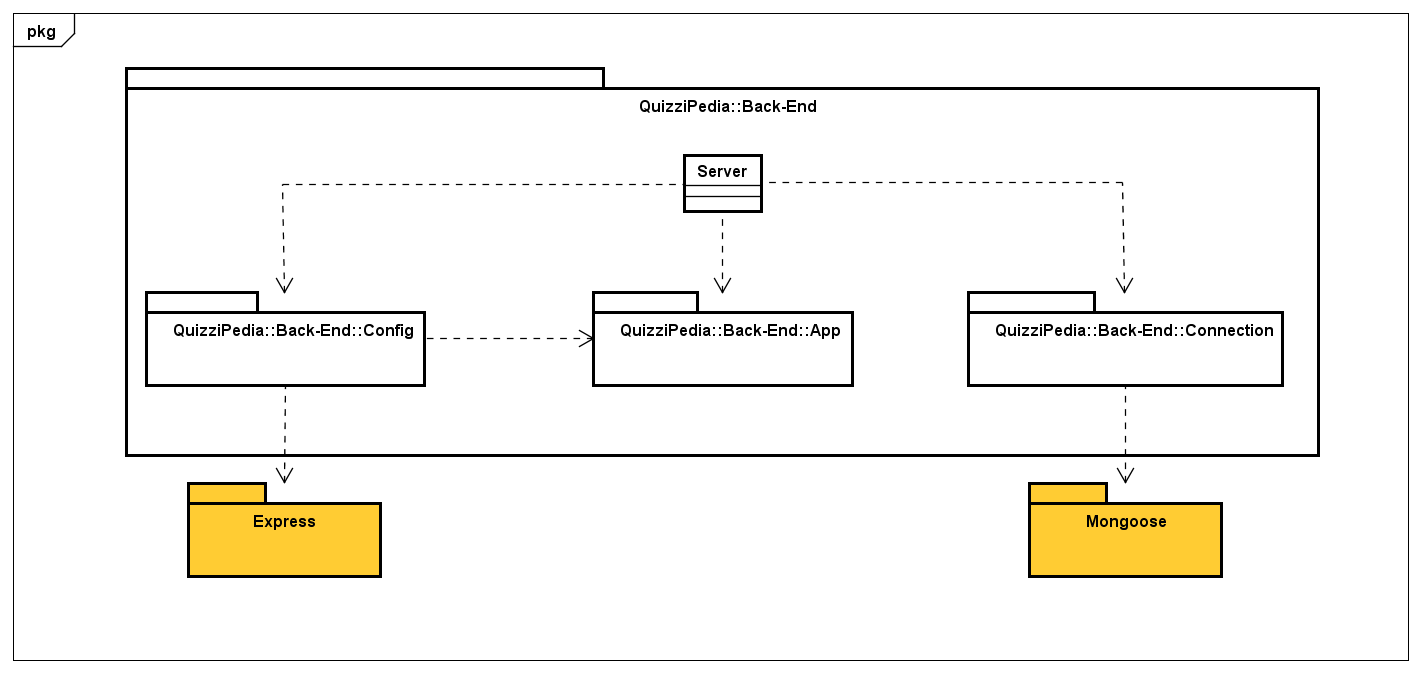
\includegraphics[scale=0.45]{UML/Package/QuizziPedia_Back-End.png}
	\caption{QuizziPedia::Back-End}
\end{figure}

	\begin{itemize}
		\item \textbf{Descrizione} \\ Package contenenti le componenti della parte back-end dell' applicazione.
		\item \textbf{Package contenuti}
		\begin{itemize}
			\item App \\
			Package\ped{G} contenente le componenti del server che implementano il \textit{pattern MVC\ped{G}}.
			\item Config \\
			Package\ped{G} contenente le componenti di configurazione del server\ped{G}.
		\end{itemize}
	\end{itemize}
\subsubsection{Classi}
	\paragraph{QuizziPedia::Back-End::Server}
	\begin{itemize}
		\item \textbf{Descrizione} \\
		Classe che avvia il server. Nello specifico apre una connessione al database tramite Mongoose, invoca il middleware\ped{G} Express\ped{G} passando un riferimento al database MongoDB\ped{G} come parametro in modo  che possa configurarsi con esso, invoca il middleware\ped{G} Passport\ped{G} ed infine si mette in ascolto su una determinata porta. E' il componente client del design pattern \textit{Chain of responsibility\ped{G}}. Utilizza i moduli Mongoose\ped{G}, Express\ped{G}, Passport\ped{G}.
		\item \textbf{Utilizzo} \\
		Utilizzo per avviare l'applicazione lato server. Inizializza, internamente al back-end, la catena di gestione delle chiamate REST\ped{G} utilizzando le classi contenute nel package \texttt{Routers}
		\item \textbf{Relazioni con altre classi}
		\item \textbf{Attributi}
		\item \textbf{Metodi}
	\end{itemize}
	